\documentclass[11pt, ngerman, fleqn, DIV=15, headinclude, BCOR=2cm]{scrreprt}

\usepackage{../../header}

\usepackage[section]{placeins}

\usepackage{csquotes}

\usepackage{tikz}
\usetikzlibrary{chains}
\usetikzlibrary{shapes.geometric}

\tikzset{device/.style={
                rectangle,
                minimum size=6mm,
                draw=black
            },
            monitor/.style={
                rectangle,
                rounded corners=2mm,
                minimum size=6mm,
                draw=black
            },
        }

\usepackage{pgfplots}
\pgfplotsset{
    compat=1.5,
    width=0.8\linewidth,
    xticklabel style={/pgf/number format/use comma},
    yticklabel style={/pgf/number format/use comma},
}

\usepgfplotslibrary{external}
\tikzexternalize

\DeclareSIUnit{\skt}{SKT}

\usepackage{booktabs}

\hypersetup{
    pdftitle=
}

\subject{Praktikumsprotokoll}
\title{$\boldsymbol\betaup$-Spektrometer}
\subtitle{Versuch P523 -- Universität Bonn}
\author{
    Lino Lemmer \\ \small{\href{mailto:l2@uni-bonn.de}{l2@uni-bonn.de}}
    \and
    Martin Ueding \\ \small{\href{mailto:mu@martin-ueding.de}{mu@martin-ueding.de}}
}

\date{\daterange{2014-04-24}{2014-04-25}}

\publishers{Tutor: Farah Noreen Afzal}

\begin{document}

\maketitle


\begin{abstract}
    In diesem Versuch kalibrieren wir ein doppeltfokussierendes $\piup
    \sqrt2$-Spektrometer mit $^{137}$Ba und bestimmen das Auflösungsvermögen.
    Wir nehmen die $\betaup$-Spektren von $^{22}$Na und $^{204}$Tl auf. Aus den
    Messdaten bestimmen wir die Maximalenergie der emittierten Teilchen.
\end{abstract}

\tableofcontents

\chapter{Theorie}

\section{Zerfallsarten}

\newcommand\betaplus{\betaup^+}
\newcommand\betaminus{\betaup^-}

Instabile Kerne können über verschiedene Kanäle zerfallen. Die für diesen
Versuch Interessanten sind die $\betaplus$- und $\betaminus$-Zerfälle sowie der
Elektroneneinfang.

Bei $\betaminus$-Zerfall passiert auf Quarkebene folgendes:
\[
    \mathrm d
    \quad\rightharpoonup\quad
    \mathrm u + \mathrm W^-
    \quad\rightharpoonup\quad
    \mathrm u + \mathrm e^- + \bar\nuup_{\mathrm e}.
\]

Auf Nukleonenebene ohne Zwischenschritt sieht der Vorgang wie folgt aus:
\[
    \mathrm n
    \quad\rightharpoonup\quad
    \mathrm p + \mathrm e^- + \bar\nuup_{\mathrm e}..
\]

Analog funktioniert der $\betaplus$-Zerfall, bei dem ein $\mathrm W^+$-Boson
ausgetauscht wird:
\[
    \mathrm p
    \quad\rightharpoonup\quad
    \mathrm n + \mathrm e^+ + \nuup_{\mathrm e}.
\]

Der Elektroneneinfang ist ein $\betaplus$-Zerfall, bei dem das Position auf der
anderen Seite der Reaktionsgleichung steht:
\[
    \mathrm p + \mathrm e^-
    \quad\rightharpoonup\quad
    \mathrm n + \nuup_{\mathrm e}.
\]

Der Kern, dessen Ladungszahl um eins verändert worden ist, wird meist in einem
angeregten Zustand hinterlassen. Diese Energie wird durch $\gammaup$-Strahlung
abgebaut.

Nach einem Elektroneneinfang ist ein Zustand mit niedriger Energie in der Hülle
unbesetzt. Elektronen aus höheren Zuständen werden in die niedrigeren Zustände
fallen und dabei charakteristische Röntgenstrahlung emittieren.

Es ist möglich, dass die Energie von einem Hüllenelektron absorbiert
wird, welches aufgrund der großen Energie vom Kern getrennt wird. Diese
Elektronen nennt man \emph{Augerelektronen}.

\section{Fermitheorie}

Im Spektrometer wird der Impuls des Elektrons durch seine Krümmung einem
Magnetfeld bestimmt. Der Krümmungsradius $\rho$ folgt schnell aus dem Ansatz
„Einstein-Lorentz-Kraft wirkt als Zentripetalkraft“:
\[
    epB = \frac{p^2}{\rho}
    \iff
    p = eB\rho.
\]

Diese Form ist auch in \parencite[§2.232]{Riezler/Kernphysikalisches}
angegeben. Da $p \propto B\rho$, kann man die Energien auch als $B\rho$-Werte
angeben, die traditionell in der veralteten Einheit \si{\gauss\centi\meter}
gemessen werden. Dies entspricht \SI{0.1}{\milli\tesla\centi\meter}, also
\si{\micro\tesla\meter}.
    
Energie und Impuls können durch folgende dimensionslose Größen ausgedrückt
werden: \parencite[(132) und (133)]{Riezler/Kernphysikalisches}
\[
    \epsilon := \frac{E}{m c^2} = 1 + \frac{E_\text{kin}}{m c^2}
    \eqnsep
    \eta := \frac{p}{m c}.
\]

Weiterhin gelten aus der speziellen Relativitätstheorie die Beziehungen:
\parencite[(134)]{Riezler/Kernphysikalisches}
\[
    \epsilon^2 = 1 + \eta^2
    \iff
    \eta = \sqrt{\epsilon^2 - 1}.
\]

Damit werden wir jetzt die erwartete Energieverteilung herleiten. Wir beginnen
mit Fermis goldener Regel \parencite[Seite~9]{Hof/Poltergeist}:
\[
    \dot N(p) \dif p = \frac{2\piup}{\hbar} \abs{\bra{\text E} H \ket{\text A}}^2 \dod n{E_0},
\]
wobei $\dot N(p) \dif p$ die Zählrate an Teilchen ist, deren Impuls im
Intervall $[p, p + \dif p]$ liegt. $H$ ist der Hamiltonoperator der
Wechselwirkung, die den Anfangszustand $\ket{\text A}$ in den Endzustand
$\ket{\text E}$ überführt. $n(E_0)$ ist die Zustandsdichte im Phasenraum. Die
Vorfaktoren und das Matrixelement ist weitestgehend energieunabhängig, so dass
wir für unsere Zwecke hier schreiben können:
\[
    \dot N(p) \dif p \propto \dod n{E_0}.
\]

Als nächstes leiten wir die Zustandsdichte im Phasenraum her. Durch die
Unbestimmtheitsrelation nimmt jeder Zustand $\ket{x, p}$ ein Phasenraumvolumen
von $(2\piup\hbar)^3$ ein. Die Anzahl der Zustände der Impulszustände bis zum
Maximalimpuls $p$, die auf der Kernvolumen $V$ beschränkt sind, sind durch
Integration über den Phasenraum gegeben:
\[
    n(p) = \frac{1}{(2\piup\hbar} \frac 43 \piup p^3 V.
\]

Dies gilt für jedes Teilchen. Da wir hier Elektron und Antineutrino betrachten
müssen, ist unsere Zustandsdichte das Produkt der zwei Zustandsdichten, da der
gesamte Phasenraum das kartesische Produkt der beiden Räume ist. Somit erhalten
wir mit $\dif n = \dif n_{\text e} \dif n_\nuup$, bis auf Vorfaktoren:
\[
    \dod n{E_0} \propto p_{\text e}^2 p_\nuup^2 \dod{p_\nuup}{E_0} \dif
    p_{\text e}.
\]

Die gesamte Energie, die beim Zerfall frei wird, ist $E_0$. Diese teilt sich
auf in die Energie, die Elektron und Neutrino jeweils bekommen. Daher gilt
natürlich $E_0 = E_{\text e} + E_\nuup$. Somit können wir das unbekannte
$p_\nuup$ ausdrücken:
\[
    p_\nuup = \frac{E_\nuup}{c} = \frac 1c \cdot (E_0 - E_{\text e}).
\]
Die Ableitung nach $E_0$ ist nur $c^{-1}$, so dass sich die Zustandsdichte zu
\[
    \dod n{E_0} \propto p^2 \cdot (E_0 - E)^2 \dif p
\]
vereinfachen lässt. Da nur noch Elektronenimpulse vorkommen, lassen wir ab hier
wieder den Index weg. Ab hier wird die Fermifunktion $F$ eingeführt, um
elektromagnetische Wechselwirkungen zwischen Kern und Elektron abbilden zu
können. Die Zustandsdichte ist nun:
\[
    \dod n{E_0} \propto F(p, Z) p^2 \cdot (E_0 - E)^2 \dif p.
\]
In dimensionslosen Einheiten ist dies:
\[
    \dod n{\epsilon_0} \propto F(\eta, Z) \eta^2 \cdot (\epsilon_0 -
    \epsilon)^2 \dif \eta.
\]

Im Experiment werden wir zuerst Impulse $p$ (oder $B\rho$) messen, die wir in
Energien umrechnen. Diese werden wir dann in dimensionslose Energien $\epsilon$
überführen. Die Fermifunktion für Natrium, die wir aus
Abbildung~\ref{fig:fermifunktion} ablesen sollen, hängt von der Energie ab. Die
Fermifunktion für Thallium, die in der Praktikumsanleitung gegeben ist, hängt
vom Impuls ab. Wir werden die bisher hergeleitete Gleichung so transformieren,
dass sie von der Energie abhängt, damit alles weitere einheitlich ist. Die
Differentiale transformieren sich nach
\parencite[(135)]{Riezler/Kernphysikalisches} wie folgt:
\[
    \eta \dif \eta = \epsilon \dif \epsilon.
\]
Das zu erwartende Spektrum ist daher:
\[
    \dot N(\epsilon) \dif \epsilon \propto F(\eta, Z) \epsilon\eta \cdot (\epsilon_0 -
    \epsilon)^2 \dif \epsilon.
\]

\begin{figure}[htbp]
    \centering
    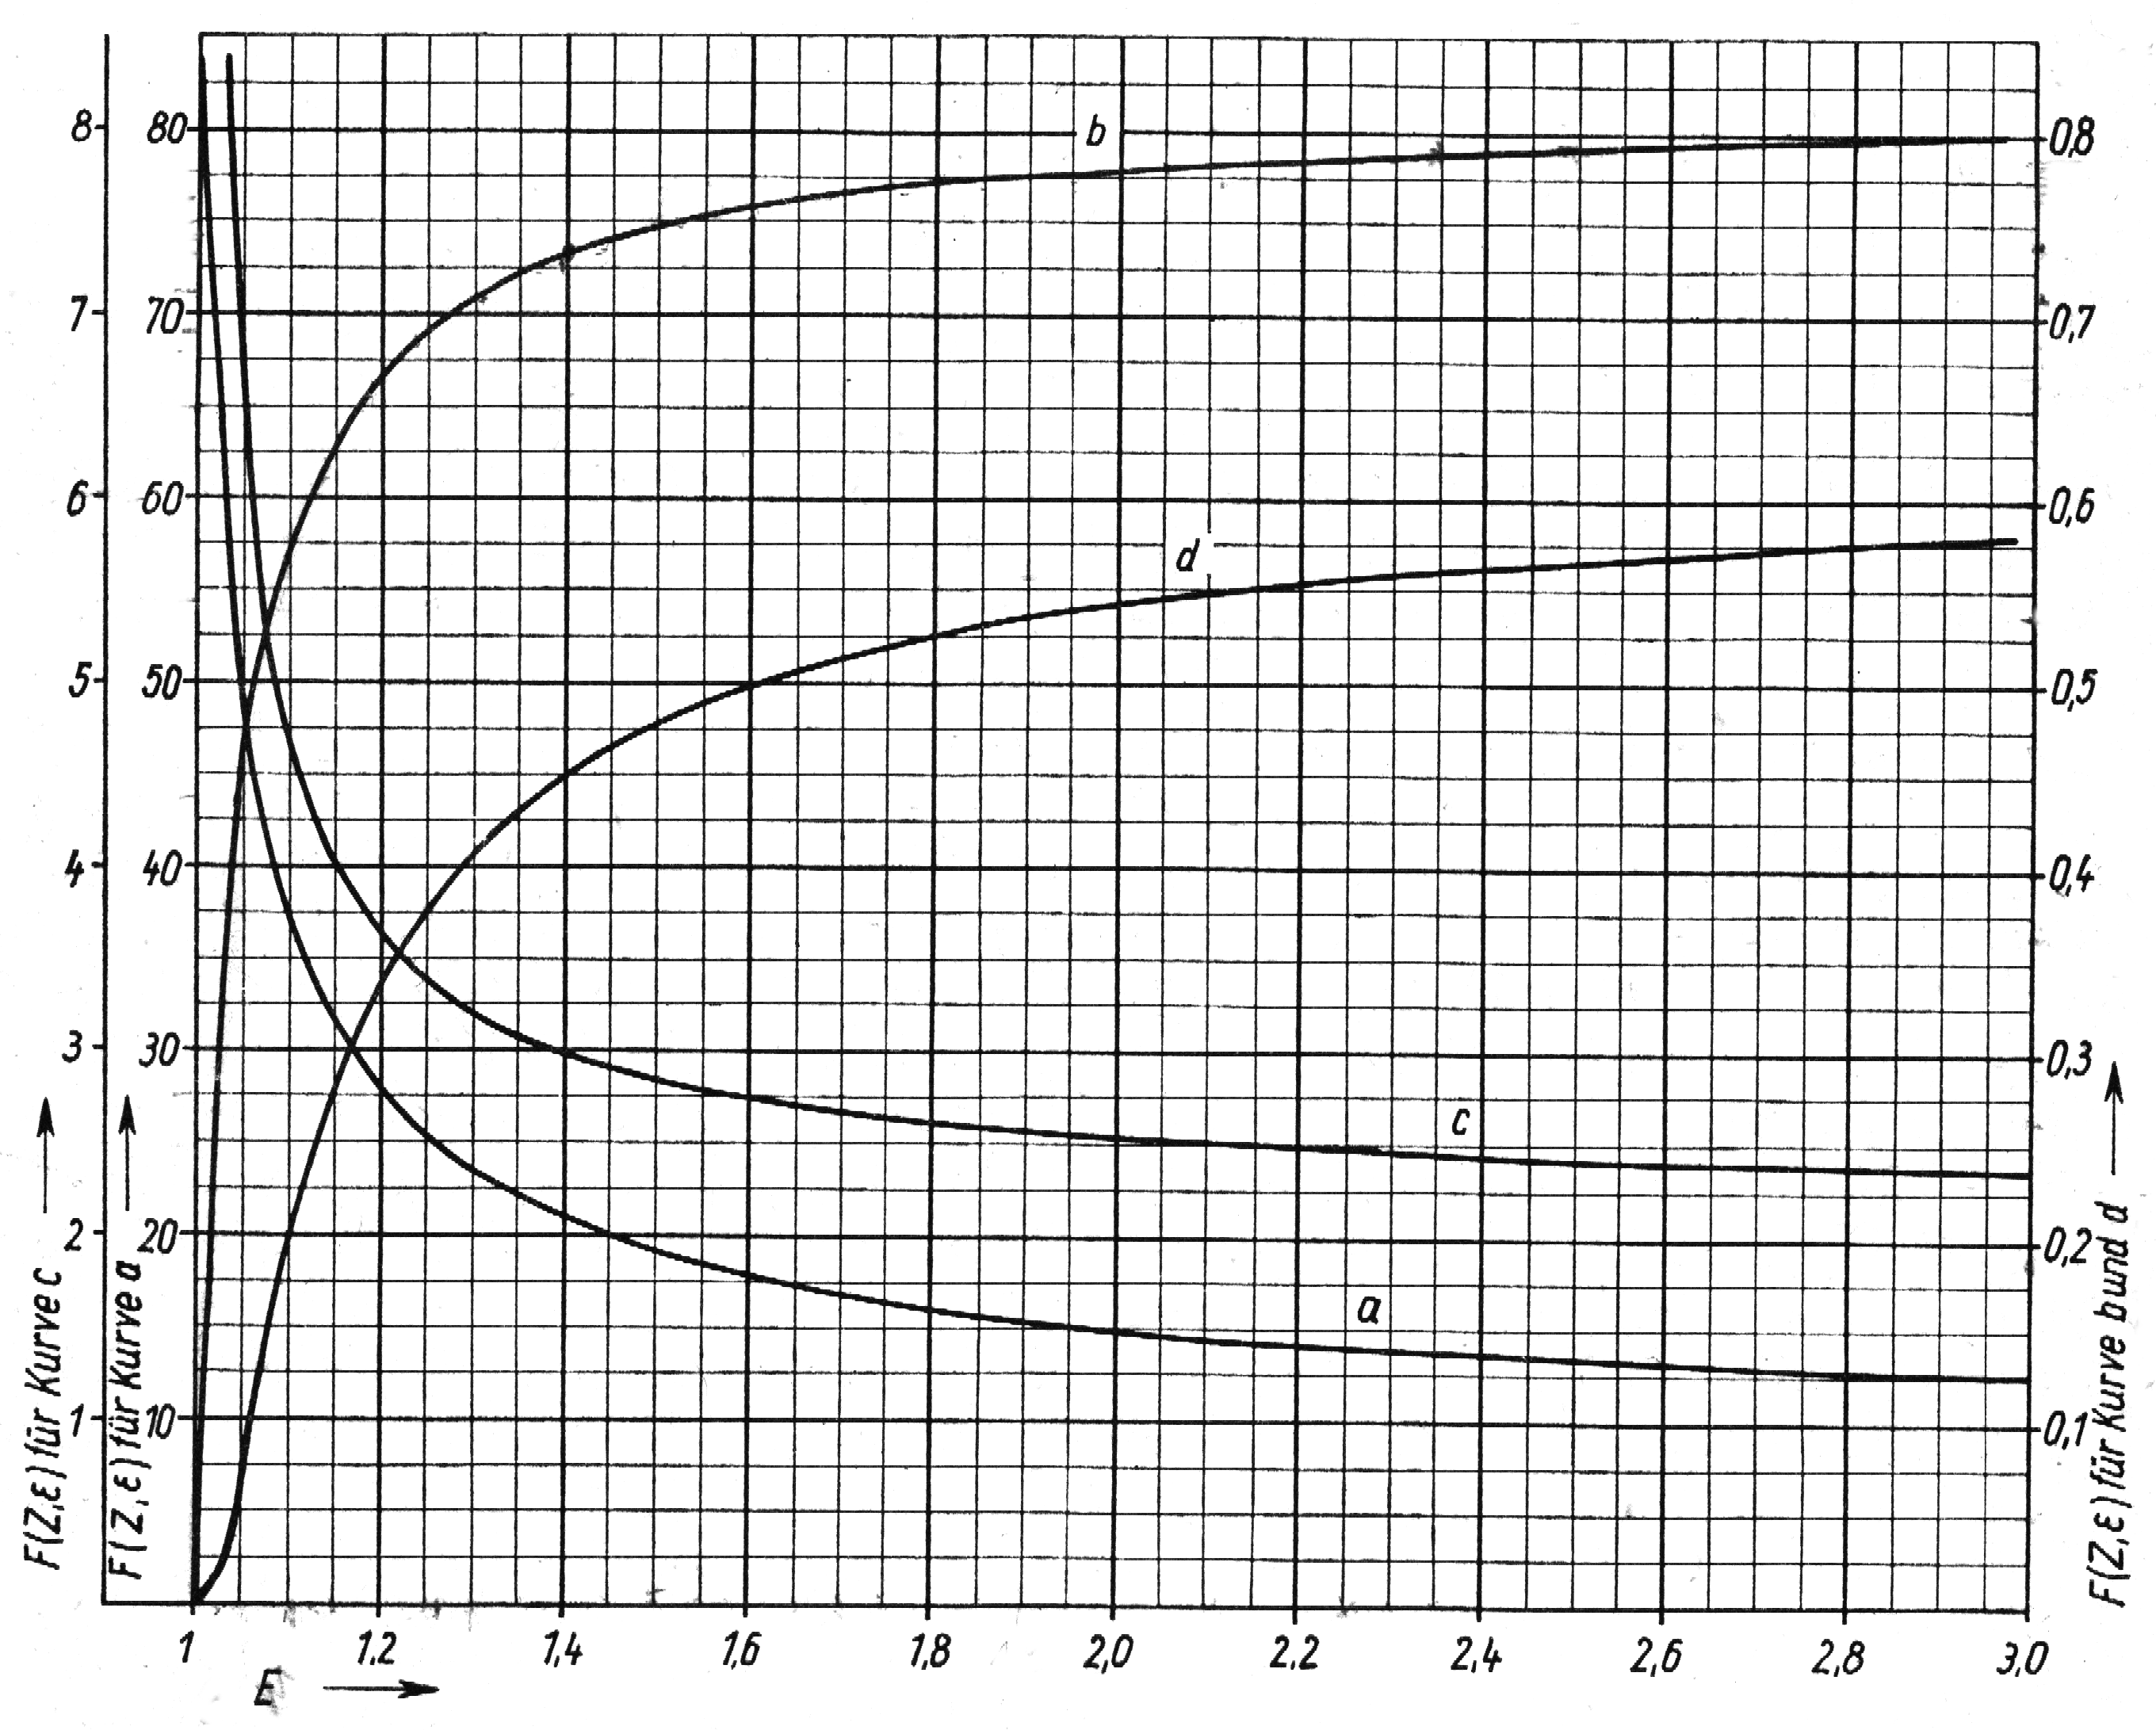
\includegraphics[width=\linewidth]{../Fermifunktion.png}
    \caption{%
        Fermi-Funktion $F(Z, \epsilon)$ für den $\betaminus$-Übergang von
        Hf$^{181}$ (Kurve a), $\betaplus$-Übergang von Na$^{22}$ (Kurve b),
        $\betaminus$- und $\betaplus$-Übergang von Cu$^{64}$ (Kurve c bzw\@.
        d). Aus \parencite[Fig. 111]{Riezler/Kernphysikalisches} mit
        freundlicher Erlaubnis des Springer-Verlags.
    }
    \label{fig:fermifunktion}
\end{figure}

\subsection{Kuriedarstellung}

In der Kuriedarstellung\footnote{Nach F.\,N.\,D\@.~Kurie, nicht Marie Curie
\parencite{wikipedia/Kurie}} trägt man nicht die Zählrate gegen die kinetische
Energie auf, sondern transformiert die Zählrate zur Größe $K$ wie folgt
\parencite[(138)]{Riezler/Kernphysikalisches}:
\begin{equation}
    K(\epsilon) = \sqrt{\frac{\dot N(\epsilon)}{F(Z, \epsilon) \eta(\epsilon)
    \epsilon}}. \label{eq:Kurie}
\end{equation}
Dadurch entsteht im Diagram eine Gerade, die die Abszisse bei $E_0$ schneidet,
sofern die Neutrinos masselos sind. Haben die Neutrinos eine endliche Masse, so
wird der Schnittpunkt bei etwas kleineren Energien liegen, da nicht die volle
Zerfallsenergie als kinetische Energie für das Elektron zur Verfügung steht.

\section{Spektrometeraufbau}

Die beiden für diese Art Versuche interessanten Spektrometer sind das
Halbkreisspektrometer und das doppeltfokussierende $\piup \sqrt
2$-Spektrometer.

Das Halbkreisspektrometer arbeitet mit einem Permanentmagneten, der die
Elektronen auf einer Kreisbahn arbeitet. Jedoch werden Elektronen mit gleicher
Energie nicht auf ganz genau auf einen Punkt fokussiert, sondern in einem
Bereich $\Deltaup x$ verschmiert
\parencite[§2.231]{Riezler/Kernphysikalisches}. Je größer der Sollradius
$\rho_0$ ist, desto besser wird die Abbildung nach 
\[
    \Deltaup x = s + \frac{j^2}{\piup^2 \rho} + \rho \phi^2,
\]
wobei $s$ und $h$ die Breite und Höhe der Probe und $\phi$ der halbe
Öffnungswinkel der Strahlen aus der Probe sind
\parencite[(123)]{Riezler/Kernphysikalisches}.

Eine bessere Fokussierung schafft das doppeltfokussierende $\piup \sqrt
2$-Spektrometer durch ein inhomogenes Magnetfeld. Man nutzt dazu
ein rotationssymmetrisches Magnetfeld mit einem radialen Gradienten. In
\parencite[§2.232]{Riezler/Kernphysikalisches} wird nun folgende Herleitung der
benötigten Radialabhängigkeit $B(\rho)$ sowie des benötigten
Spektrometerwinkels $\Phi$ gegeben:

Sei der Sollkreis mit Radius $\rho_0$ durch den Elektronenimpuls $p$ durch $p =
e B \rho_0$ bestimmt. Ein Teilchen, dass in einem Winkel $\phi_\rho$ zum
Sollkreis von dessen Rand startet, schneidet ihn wieder am Rand um den Winkel
$\Phi_\rho$ versetzt. Für diesen Winkel gilt für kleine $\phi_\rho$:
\parencite[(125)]{Riezler/Kernphysikalisches}
\[
    \Phi_\rho = \piup \cdot \del{1 + \frac{\rho_0}{B(\rho_0)} \dpd B
    \rho}^{-\frac 12}.
\]

In der axialen Richtung gilt eine ähnliche Bedingung:
\parencite[(126)]{Riezler/Kernphysikalisches}
\[
    \Phi_z = \piup \cdot \del{- \frac{\rho_0}{B(\rho_0)} \dpd B
    \rho}^{-\frac 12}.
\]

Aus diesen beiden Gleichungen folgt laut den Autoren nun die Beziehung:
\parencite[(127)]{Riezler/Kernphysikalisches}
\[
    \frac1{\Phi_\rho^2} + \frac1{\Phi_z^2} = \frac1{\piup^2}.
\]

Mit der Bedingung, dass diese beiden Winkel gleich sein müssen ist die Lösung
der entsprechenden Differentialgleichung:
\parencite[(129)]{Riezler/Kernphysikalisches}
\[
    \Phi = \piup \sqrt 2 \approx \SI{256}{\degree}.
\]

Daher hat dieses Spektrometer seinen Namen.

Das Spektrometer hat noch eine Dispersion, so dass die Impulsintervalle nicht
gleich groß sind. Die Dispersion ist angegeben als:
\parencite[(130)]{Riezler/Kernphysikalisches}
\[
    \gamma = \frac{4 \rho_0}{B \rho},
\]
weshalb die Messwerte mit $\gamma$ zu multiplizieren sind. Da wir die Energie
mit den Konversionslinien eichen werden, ist jede zum Impuls proportionale
Größe geeignet \parencite[§P523.5.4]{physik512-Anleitung}.

\section{Detektoren}

In diesem Versuch benötigen wir im Detektor keine Energieinformation, da wir
diese bereits durch das Magnetfeld erhalten. Wichtiger ist, dass alle
Elektronen detektiert werden und die Totzeit gering ist.

Ein möglicher Detektor ist das Geiger-Müller Zählrohr, bei dem eintretende
Teilchen ein Gas ionisieren und somit eine Hochspannungsentladung auslösen. Der
Strompuls kann verstärkt und gezählt werden.

Eine Diode, die in Sperrrichtung betrieben wird, eignet sich ebenfalls als
Detektor. Tritt ein Elektron in den die Sperrzone ein, erzeugt es dort freie
Ladungsträger (Elektronen und Löcher), die dann ebenfalls zu einem Strompuls
führen.

\section{Hysterese}

Eisen ist ferromagnetisch, es behält seine Magnetisierung $M$ auch ohne
angelegtes Magnetfeld $H$ bei. Legt man Eisen in ein Magnetfeld und erhöht die
Flussdichte bis zu einem Maximum (so dass die Magnetisierung in Sättigung geht)
und erniedrigt wieder bis $H = 0$, so nennt man die verbleibende Magnetisierung
\emph{Remanenzfeld}. Dieser Effekt ist isotrop, so dass man durch den
Mittelwert der beiden Remanenzfeldstärken die neutrale Mitte herausfinden kann.

Möchte man einen Ferromagneten entmagnetisieren, muss man das Magnetfeld, indem
sich der Ferromagnet befindet, in mehreren Durchläufen zwischen dem positiven
und negativen Maximum regeln, wobei ab dem zweiten Durchlauf der
Betrag der maximalen Magnetfeldstärke reduziert wird. Dadurch wird das
Remanenzfeld bei jedem Durchlauf schwächer, bis am Ende verschwindet. Diesen
Vorgang nennt man \emph{Hysterese}. Dieser Vorgang ist in
Abbildung~\ref{fig:hysterese} dargestellt.

\begin{figure}[htbp]
    \centering
    \begin{tikzpicture}
        \begin{axis}[
                width=\linewidth,
                height=0.7\linewidth,
                xlabel=Spulenstrom / wilk.\,Einh.,
                ylabel=Flussdichte / wilk.\,Einh.,
                grid=major,
            ]
            \addplot[black] table [x index=1, y index=2]{../Daten/data.txt};
        \end{axis}
    \end{tikzpicture}
    \caption{%
        Hysteresekurve von Eisen. Messdaten aus \parencite{Ueding/248}.
    }
    \label{fig:hysterese}
\end{figure}

\chapter{Durchführung}

\section{Offsetspannung}

Wir erhöhen, zunächst ohne Strahler, den Magnetstrom bis die Magnetisierung
in Sättigung geht. Die Hallsonde zeigt
\num{-183.2(3)}\footnote{\erklaerungFehlerNotation} Skalenteile (von nun an
\si{\skt}) an. Wir notieren die
Remanenz. Nach dem Umpolen erreichen wir eine Sättigung von
\SI{196.0(3)}{\skt}. Unsere Messwerte sind in Tabelle~\ref{tab:remanenz} zu
sehen.

\begin{table}[htbp]
    \centering
    \begin{tabular}{SS}
        {Untere Remanenz/\si{\skt}} & {Obere Remanenz/\si{\skt}}\\
        \midrule
        %< for a, b in tab_remanenz: ->%
        << a >> & << b >> \\
        %< endfor ->%
    \end{tabular}
    \caption{%
        Untere und obere Remanenz der Spektrometer-Hysterese.
    }
    \label{tab:remanenz}
\end{table}

Der Mittelwert der Differenzen zwischen oberer und unterer Remanenz ist die
Offsetspannung. Wir erhalten \SI{<< hall_offset >>}{\skt}.

\section{Kalibrierung des $\betaup$-Spektrometers}

Wir setzen die Caesiumprobe ein und evakuieren das Spektrometer wieder. Den
Magnetstrom polen wir so, dass der Detektor Ereignisse anzeigt. Nun messen
wir zunächst bei \SI{4}{\percent} Transmission \SI{40}{\second} lang die
Anzahl der Ereignisse bei verschiedenen Magnetisierungen. Diese gehen wir in
\SI{10}{\skt}-Schritten ab. Unsere Messwerte sind in
Tabelle~\ref{tab:Cs-40-kompl} zu sehen.

\begin{table}[htbp]
    \centering
    \begin{tabular}{SS}
        {Hall-Spannung/\si{\skt}} & {Anzahl d. Ereignisse} \\
        \midrule
        %< for a, b in Cs_40s_kompl_mess: ->%
        << a >> & << b >> \\
        %< endfor ->%
    \end{tabular}
    \caption{%
        Messwerte zur Kalibrierung des Spektrometers. Probe: ${}^{137}$Cs,
        Zeit: \SI{40}{\second}, Transmission: \SI{4}{\percent}.
    }
    \label{tab:Cs-40-kompl}
\end{table}

Die Erhöhung der Zählrate im Bereich zwischen \SI{89}{\skt} und
\SI{129}{\skt} ist das normale $\betaup$-Spektrum, der Peak bei
\SI{159.3}{\skt} enthält die Konversionslinien. Um diese aufzulösen,
vermessen wir den Bereich \SIrange{149}{168}{\skt} in \SI{.5}{\skt}-Schritten
zunächst mit \SI{4}{\percent} Transmission und \SI{40}{\second} Messdauer,
danach mit \SI{1}{\percent} Transmission und \SI{100}{\second} Messdauer je
Intervall. Die Messdaten finden sich in den Tabellen~\ref{tab:Cs-40-aussch}
und \ref{tab:Cs-100}.

\begin{table}[htbp]
    \centering
    \begin{tabular}{SS}
        {Hall-Spannung/\si{\skt}} & {Anzahl d. Ereignisse} \\
        \midrule
        %< for a, b in Cs_40s_ausschn_mess: ->%
        << a >> & << b >> \\
        %< endfor ->%
    \end{tabular}
    \caption{%
        Messwerte zur Kalibrierung des Spektrometers. Probe: ${}^{137}$Cs,
        Zeit: \SI{40}{\second}, Transmission: \SI{4}{\percent}.
    }
    \label{tab:Cs-40-aussch}
\end{table}

\begin{table}[htbp]
    \centering
    \begin{tabular}{SS}
        {Hall-Spannung/\si{\skt}} & {Anzahl d. Ereignisse} \\
        \midrule
        %< for a, b in Cs_100s_mess: ->%
        << a >> & << b >> \\
        %< endfor ->%
    \end{tabular}
    \caption{%
        Messwerte zur Kalibrierung des Spektrometers. Probe: ${}^{137}$Cs,
        Zeit: \SI{100}{\second}, Transmission: \SI{1}{\percent}.
    }
    \label{tab:Cs-100}
\end{table}

\section{Vermessung des ${}^{204}$Tl- und ${}^{22}$Na-Spektrums}

Wir wählen als nächstes die Thallium-Probe aus, da diese wie das Caesium ein
$\betaup^-$-Strahler ist und wir so das Magnetfeld nicht umpolen müssen. Wir
stellen zunächst eine Messdauer von \SI{100}{\second}, bei \SI{4}{\percent}
Transmission ein, um einen groben Bereich für das Maximum des Spektrums zu
% TODO Werte einfügen.
finden. Dieses liegt bei etwa \SIrange{}{}{\skt}. Wir wählen in diesem Bereich
eine Hall-Spannung aus, um uns für eine Messdauer für die Spektrumsaufnahme
zu entscheiden. Wir wählen \SI{80}{\second} aus, da bei dieser Zeit das Maximum
über \num{1000} Ereignisse aufweist. Die Messwerte finden sich in
Tabelle~\ref{tab:Tl-80}. Als Untergrund wählen wir, wegen fehlender Messung,
\num{<< Tl_80s_untergrund >>} Ereignisse.

\begin{table}[htbp]
    \centering
    \begin{tabular}{SS}
        {Hall-Spannung/\si{\skt}} & {Anzahl d. Ereignisse} \\
        \midrule
        %< for a, b in Tl_80s_mess: ->%
        << a >> & << b >> \\
        %< endfor ->%
    \end{tabular}
    \caption{%
        Messwerte zur Bestimmung des $\betaup$-Spektrums. Probe: ${}^{204}$Tl,
        Zeit: \SI{80}{\second}, Transmission: \SI{4}{\percent}.
    }
    \label{tab:Tl-80}
\end{table}

Im Anschluss polen wir das Magnetfeld um und setzen die Natrium-Probe ein. Wir
verfahren genauso wie bei der Thallium-Probe und wählen als Messdauer
\SI{200}{\second}. Die Messwerte sind in Tabelle~\ref{tab:Na-200} zu sehen. Als
Untergrund haben wir \num{<< Na_200s_untergrund >>} Ereignisse gemessen.

\begin{table}[htbp]
    \centering
    \begin{tabular}{SS}
        {Hall-Spannung/\si{\skt}} & {Anzahl d. Ereignisse} \\
        \midrule
        %< for a, b in Na_200s_mess: ->%
        << a >> & << b >> \\
        %< endfor ->%
    \end{tabular}
    \caption{%
        Messwerte zur Bestimmung des $\betaup$-Spektrums. Probe: ${}^{22}$Na,
        Zeit: \SI{200}{\second}, Transmission: \SI{4}{\percent}.
    }
    \label{tab:Na-200}
\end{table}

\chapter{Auswertung}

\section{Impulseichung des $\betaup$-Spektrometers}

Zur Weiterverarbeitung unserer Daten müssen wir, da die
ausgemessenen Impulsintervalle proportional zum Impuls selbst sind, die
Zählrate wiederum durch eine zum Impuls proportionale Größe, in unserem Fall
die um den Offset korrigierte Hall-Spannung, teilen. Die Entsprechenden Plots
sind in den Abbildungen~\ref{fig:Cs-40s-ausschn} bis \ref{fig:Na-200s} zu sehen,
wobei wir die erste, grobe Messung ausgelassen haben, da diese nur zum Finden
des Peak-Bereiches gemacht wurde.

%\begin{figure}[htpb]
%    \centering
%    \begin{tikzpicture}
%        \begin{axis}[
%                width=.7\linewidth,
%                height=.4\linewidth,
%                xlabel=Hallspannung/Skt.,
%                ylabel=Ereignisse,
%            ]
%            \addplot[error bars/.cd,
%                x dir=both, x explicit,
%                y dir=both, y explicit
%            ]
%            table[x error index=2, y error index=3] {../_build/01_Cs_40s_bearb.txt};
%        \end{axis}
%    \end{tikzpicture}
%    \caption{%
%        $\betaup$-Spektrum von ${}^{137}$Cs bei \SI{40}{\second}
%        Messdauer und \SI{4}{\percent} Transmission
%    }
%    \label{fig:Cs-40s-vollst}
%\end{figure}

\begin{figure}[htpb]
    \centering
    \begin{tikzpicture}
        \begin{axis}[
                width=.7\linewidth,
                height=.4\linewidth,
                xlabel=$U_\text{Hall}$/\si{\skt},
                ylabel=Ereignisse,
                no markers,
                grid=major,
            ]
            \addplot[scatter, only marks,
                error bars/.cd,
                x dir=both, x explicit,
                y dir=both, y explicit
            ]
            table[x error index=2, y error index=3] {../_build/02_Cs_40s_bearb.txt};
            \addplot[black] table {../_build/fit_konversion_40_K.txt};
            \addplot[black] table {../_build/fit_konversion_40_L.txt};
        \end{axis}
    \end{tikzpicture}
    \caption{%
        $\betaup$-Spektrum von ${}^{137}$Cs bei \SI{40}{\second}
        Messdauer und \SI{4}{\percent} Transmission
    }
    \label{fig:Cs-40s-ausschn}
\end{figure}

\begin{figure}[htpb]
    \centering
    \begin{tikzpicture}
        \begin{axis}[
                width=.7\linewidth,
                height=.4\linewidth,
                xlabel=$U_\text{Hall}$/\si{\skt},
                ylabel=Ereignisse,
                no markers,
                grid=major,
            ]
            \addplot[scatter, only marks,
                error bars/.cd,
                x dir=both, x explicit,
                y dir=both, y explicit
            ]
            table[x error index=2, y error index=3] {../_build/03_Cs_100s_bearb.txt};
            \addplot[black] table {../_build/fit_konversion_100_K.txt};
            \addplot[black] table {../_build/fit_konversion_100_L.txt};
        \end{axis}
    \end{tikzpicture}
    \caption{%
        $\betaup$-Spektrum von ${}^{137}$Cs bei \SI{100}{\second}
        Messdauer und \SI{1}{\percent} Transmission
    }
    \label{fig:Cs-100s}
\end{figure}

\begin{figure}[htpb]
    \centering
    \begin{tikzpicture}
        \begin{axis}[
                width=.7\linewidth,
                height=.4\linewidth,
                xlabel=$U_\text{Hall}$/\si{\skt},
                ylabel=Ereignisse,
                grid=major,
            ]
            \addplot[error bars/.cd,
                x dir=both, x explicit,
                y dir=both, y explicit
            ]
            table[x error index=2, y error index=3] {../_build/04_Tl_80s_bearb.txt};
        \end{axis}
    \end{tikzpicture}
    \caption{%
        $\betaup$-Spektrum von ${}^{204}$Tl bei \SI{80}{\second}
        Messdauer und \SI{4}{\percent} Transmission
    }
    \label{fig:Tl-80s}
\end{figure}

\begin{figure}[htpb]
    \centering
    \begin{tikzpicture}
        \begin{axis}[
                width=.7\linewidth,
                height=.4\linewidth,
                xlabel=$U_\text{Hall}$/\si{\skt},
                ylabel=Ereignisse,
                grid=major,
            ]
            \addplot[error bars/.cd,
                x dir=both, x explicit,
                y dir=both, y explicit
            ]
            table[x error index=2, y error index=3] {../_build/05_Na_200s_bearb.txt};
        \end{axis}
    \end{tikzpicture}
    \caption{%
        $\betaup$-Spektrum von ${}^{22}$Na bei \SI{200}{\second}
        Messdauer und \SI{4}{\percent} Transmission
    }
    \label{fig:Na-200s}
\end{figure}

Zur Impulseichung muss der Impuls für die K- und L-Konversionslinie berechnet
werden. Die Energie des emittierten $\gammaup$-Quants beim Übergang des
${}^{137}$Cs in seinen Grundzustand ist $E_\gammaup = \SI{<< energie_gamma
>>}{\kilo\electronvolt}$. Die Bindungsenergien der K- und L-Elektronen sind
$E_\mathrm{K} = \SI{<< energie_K_bindung >>}{\kilo\electronvolt}$,
$E_\mathrm{L,I} = \SI{<< energie_L_bindung_1 >>}{\kilo\electronvolt}$,
$E_\mathrm{L,II} = \SI{<< energie_L_bindung_2 >>}{\kilo\electronvolt}$ und
$E_\mathrm{L,III} = \SI{<< energie_L_bindung_3 >>}{\kilo\electronvolt}$. Da das
Spektrometer die L-Konversionslinie nicht auflösen kann, bilden wir den
Mittelwert und erhalten so eine Bindungsenergie von $E_\mathrm{L} = \SI{<<
energie_L_bindung >>}{\kilo\electronvolt}$. Die Differenz aus
$\gammaup$- und Bindungsenergie ergibt die Energie des Elektrons. Diese rechnen
wir mit 
\[
    \eta = \sqrt{\del{\frac{E_\gammaup-E_\text{K,L}}{m_\text{e}c^2}}^2-1}
\]
in Impulse in dimensionslosen Einheiten um. Wir erhalten $\eta_\text{K} = \num{<<
impuls_K_konversion >>}$ und $\eta_\text{L} = \num{<< impuls_L_konversion >>}$.
Der Impuls ist in Abbildung~\ref{fig:impulseichung} gegen die Peakschwerpunkte
aufgetragen. Für die Anpassung ergibt sich
\[
    \eta = \del{\SI{<< fit_impulseichung_steigung >>}{\per\skt}} \cdot
    U_\text{Hall} + \del{\num{<< fit_impulseichung_offset >>}},
\]
wobei der Nullpunkt als weiterer Datenpunkt berücksichtigt worden ist. Die
Anpassung sieht aufgrund des Ausschnittes sehr schlecht aus, jedoch sind die
Residuen in Relation recht klein. Wir haben hier diesen Ausschnitt gewählt, da
ansonsten die Fehlerbalken an den Messwerten nicht mehr zu sehen wären.

\begin{figure}[htpb]
    \centering
    \begin{tikzpicture}
        \begin{axis}[
                width=.7\linewidth,
                height=.4\linewidth,
                xlabel=$U_\text{Hall}$/\si{\skt},
                ylabel=$\eta$,
                no markers,
                grid=major,
            ]
            \addplot[scatter, only marks,
                error bars/.cd,
                x dir=both, x explicit,
                y dir=both, y explicit
            ]
            table[x error index=2, y error index=3] {../_build/impulseichung_data.txt};
            \addplot[black] table {../_build/fit_impulseichung.txt};
        \end{axis}
    \end{tikzpicture}
    \caption{%
        Anpassung zur Impulseichung des Spektrometers
    }
    \label{fig:impulseichung}
\end{figure}

Wir benutzen nun die Anpassung um die Hallspannungen aus dem Thallium und
Natriumspektrum in dimensionslose Impulse umzuwandeln. Zudem berechnen wir mit
Gleichung~\eqref{eq:Kurie} den $K$-Wert zu den Impulsen und Zählraten. Dazu
benötigen wir noch die Fermifunktion der beiden Materialien. Wir haben dazu die
Werte aus Tabelle~\ref{tab:fermi_Tl} und \ref{tab:fermi_Na} linear interpoliert
um so den Fermifaktor für beliebige Impulse berechnen zu können.

\begin{table}[htpb]
    \centering
    \begin{tabular}{SS}
        {$\eta$} & {$F$}\\
        \midrule
        %< for a, b in fermi_04_Tl: ->%
        << a >> & << b >> \\
        %< endfor ->%
    \end{tabular}
    \caption{%
        Fermifunktion für Thallium \parencite[Tabelle
        P523.1]{physik512-Anleitung}.
    }
    \label{tab:fermi_Tl}
\end{table}

\begin{table}[htpb]
    \centering
    \begin{tabular}{SS}
        {$\epsilon$} & {$F$}\\
        \midrule
        %< for a, b in fermi_05_Na: ->%
        << a >> & << b >> \\
        %< endfor ->%
    \end{tabular}
    \caption{%
        Fermifunktion für Natrium. Hier wurden einfach abzulesende Punkte aus
        Abbildung~\ref{fig:fermifunktion} genommen.
    }
    \label{tab:fermi_Na}
\end{table}

Die so berechneten Werte sind in den Tabellen~\ref{tab:Kurie_Tl} und
\ref{tab:Kurie_Na} zu sehen.
 
\begin{table}[htpb]
    \centering
    \begin{tabular}{SS}
        {$\eta$} & {$K$}\\
        \midrule
        %< for a, b in Kurie_04_Tl: ->%
        << a >> & << b >> \\
        %< endfor ->%
    \end{tabular}
    \caption{%
        Dimensionslose Impulse und $K$-Wert des Betaspektrums von Thallium.
    }
    \label{tab:Kurie_Tl}
\end{table}

\begin{table}[htpb]
    \centering
    \begin{tabular}{SS}
        {$\epsilon$} & {$K$}\\
        \midrule
        %< for a, b in Kurie_05_Na: ->%
        << a >> & << b >> \\
        %< endfor ->%
    \end{tabular}
    \caption{%
        Dimensionslose Energie und $K$-Wert des Betaspektrums von Natrium
    }
    \label{tab:Kurie_Na}
\end{table}


\begin{figure}[htpb]
    \centering
    \begin{tikzpicture}
        \begin{axis}[
                width=.7\linewidth,
                height=.4\linewidth,
                xlabel=$\epsilon$,
                ylabel=$K(\epsilon)$,
                no markers,
                grid=major,
            ]
            \addplot[scatter, only marks,
                error bars/.cd,
                x dir=both, x explicit
            ]
            table[x error index=2] {../_build/Kurie_04_Tl.txt};
            \addplot[black] table {../_build/fit_kurie_04_Tl.txt};
        \end{axis}
    \end{tikzpicture}
    \caption{%
        Kurie-Plot für ${}^{204}$Tl
    }
    \label{fig:kurie-Tl}
\end{figure}

\begin{figure}[htpb]
    \centering
    \begin{tikzpicture}
        \begin{axis}[
                width=.7\linewidth,
                height=.4\linewidth,
                xlabel=$\epsilon$,
                ylabel=$K(\epsilon)$,
                no markers,
                grid=major,
            ]
            \addplot[scatter, only marks,
                error bars/.cd,
                x dir=both, x explicit
            ]
            table[x error index=2] {../_build/Kurie_05_Na.txt};
            \addplot[black] table {../_build/fit_kurie_05_Na.txt};
        \end{axis}
    \end{tikzpicture}
    \caption{%
        Kurie-Plot für ${}^{22}$Na
    }
    \label{fig:kurie-Na}
\end{figure}

Die Werte sind samt Anpassungsgeraden in den Abbildungen~\ref{fig:kurie-Tl} und
\ref{fig:kurie-Na} zu sehen. Aus deren Nullstellen erhält man die
Maximalenergie der emittierten Teilchen.  Da bei beiden Messungen einige
Messwerte deutlich von einer Geraden abwichen, haben wir, um eine vernünftige
Anpassung zu bekommen, beim Thallium die ersten beiden und den letzten, und
beim Natrium die ersten fünf und den letzten Datenpunkt ausgelassen.

Im Fall vom Thallium erhielten wir $\epsilon_\text{max} = \num{<<
epsilon_max_04_Tl >>}$, was einer Energie von $E_\text{max} = \SI{<<
E_max_04_Tl >>}{\kilo\electronvolt}$ entspricht.  Beim Natrium finden wir
$\epsilon_\text{max} = \num{<< epsilon_max_05_Na >>}$, oder $E_\text{max} =
\SI{<< E_max_05_Na >>}{\kilo\electronvolt}$. 

\section{Auflösungsvermögen}

Das Auflösungsvermögen des Spektrometers kann man mit
\[
    \frac{\eta_\text{mean}}{\Delta \eta_\text{FWHM}}
\]
berechnen, wobei $U_\text{mean}$ den Peakschwerpunk und $\Delta
U_\text{FWHM}$ die Peakbreite auf halber Maximalhöhe bezeichnen. Die
Auflösungsvermögen für die \SI{40}{\second}- und für die
\SI{100}{\second}-Messung findet man in Tabelle~\ref{tab:auflösung_40},
bzw. \ref{tab:auflösung_100}.

\begin{table}[hbtp]
    \centering
    \begin{tabular}{SSS}
        {$\eta_\text{mean}$} & {$\Delta \eta_\text{FWHM}$} &
        {Auflösungsvermögen} \\
        \midrule
        %< for a, b, c in aufloesung_40s: ->%
        << a >> & << b >> & << c >> \\
        %< endfor ->%
    \end{tabular}
    \caption{%
        Auflösungsvermögen für die \SI{40}{\second} Messung am Caesium
    }
    \label{tab:auflösung_40}
\end{table}

\begin{table}[hbtp]
    \centering
    \begin{tabular}{SSS}
        {$\eta_\text{mean}$} & {$\Delta \eta_\text{FWHM}$} &
        {Auflösungsvermögen} \\
        \midrule
        %< for a, b, c in aufloesung_100s: ->%
        << a >> & << b >> & << c >> \\
        %< endfor ->%
    \end{tabular}
    \caption{%
        Auflösungsvermögen für die \SI{100}{\second} Messung am Caesium
    }
    \label{tab:auflösung_100}
\end{table}

\chapter{Ergebnis}

Die Maximalenergie für Natrium haben wir zu \SI{<< E_max_05_Na
>>}{\kilo\electronvolt} bestimmt. Der $Q$-Wert aus dem Zerfallsdiagramm in der
Anleitung ist \SI{2842.1}{\kilo\electronvolt}, der Literaturwert für die
Maximalenergie ist jedoch \SI{545.7(5)}{\kilo\electronvolt}
\parencite{Beck/Positronenspektrum}.

Für Thallium haben wir eine Maximalenergie von \SI{<< E_max_04_Tl
>>}{\kilo\electronvolt} bestimmt. Hier liegt der Literaturwert bei
\SI{763.70}{\kilo\electronvolt}.

Dies bedeutet, dass bei Natrium die Anpassungsgerade zu flach ist, sie müsste
etwas steiler abfallen. Wenn man die letzten Datenpunkte betrachtet, so deuten
die auf eine geringere Maximalenergie hin.

Bei Thallium haben wir einen Datenpunkt, der fast bei $K = 0$ liegt. Jedoch
schwanken die umgerechneten Werte recht stark um die Ausgleichsgerade. Selbst
wenn die Steigung anders ist, wird der Schnittpunkt mit der Abszisse nicht
stark verändert.

Bei beiden Messungen müssen also noch systematische Effekte hinzukommen, da die
im Vergleich zu unseren Fehlern sehr große Abweichungen nicht nur durch die
Anpassung erklärt werden kann. Mögliche Fehlerquellen könnten die Interpolation
der Fermifunktion, Hystereseeffekte im Magneten und kurzfristige
Temperaturschwankungen im Magneten sein.

\IfFileExists{\bibliographyfile}{
    \printbibliography
}{}

\end{document}

% vim: spell spelllang=de tw=79
